\chapter{System Design}
\section{User Interface (UI) Design}
Budgetbeam's UI is built for modern accessibility and financial clarity.

\begin{figure}[h!]
    \centering
    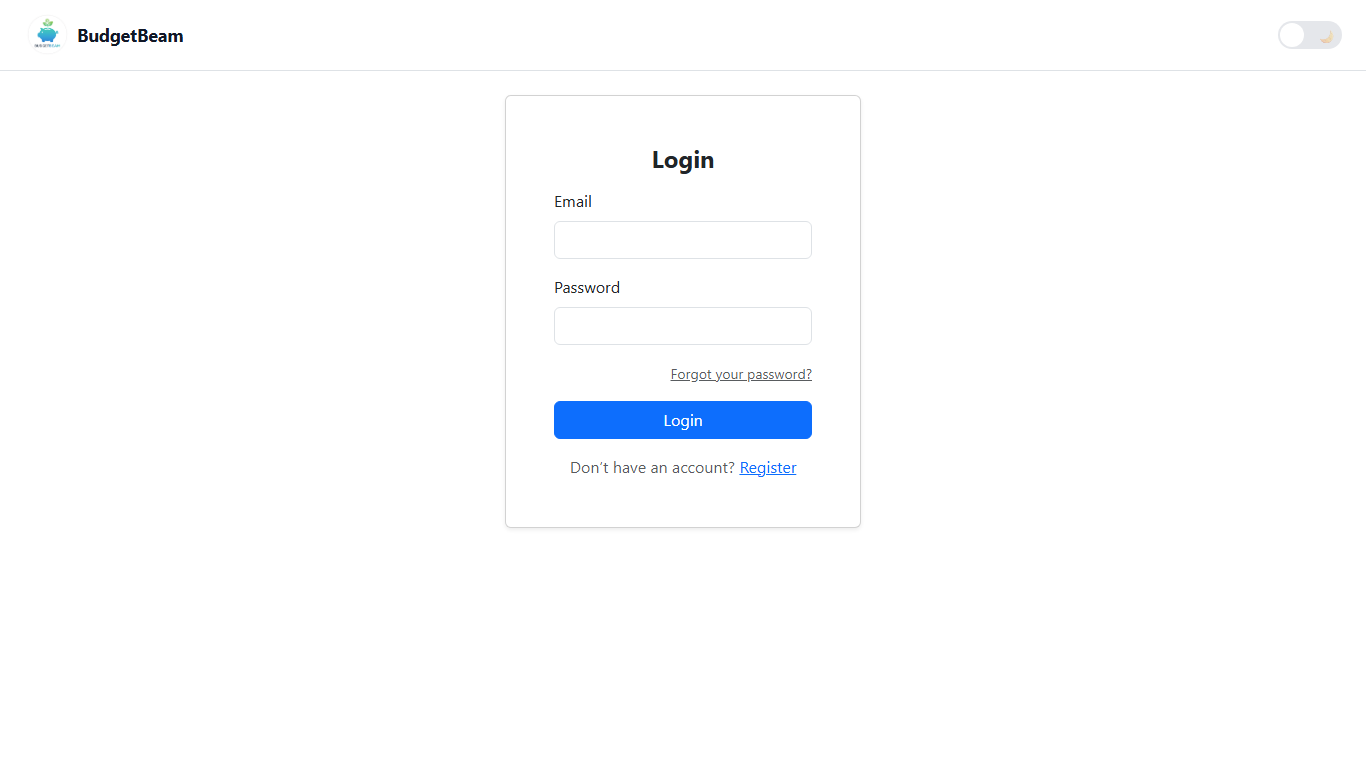
\includegraphics[width=\textwidth]{login_ui.png}
    \caption{Budgetbeam Secured Login Interface}
\end{figure}

\begin{figure}[h!]
    \centering
    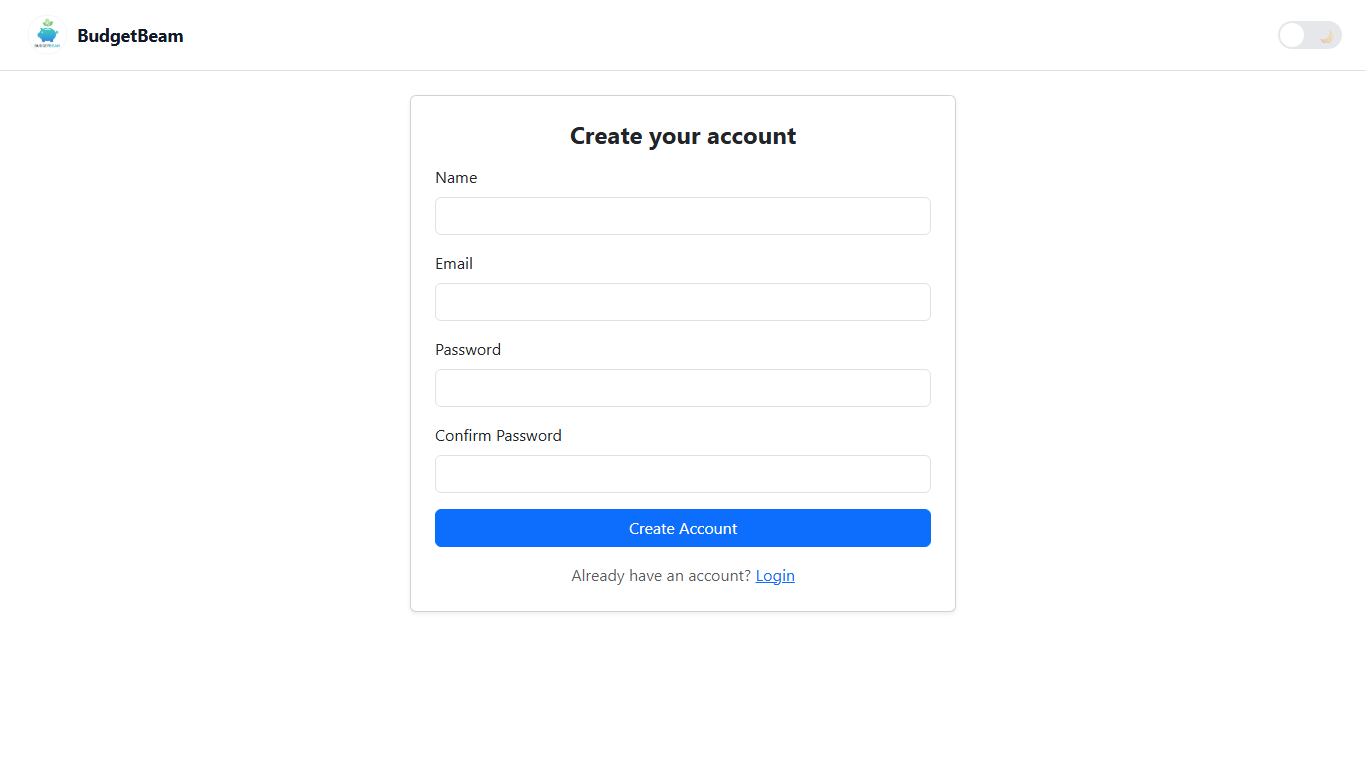
\includegraphics[width=0.85\textwidth]{register_ui.png}
    \caption{Budgetbeam Account Registration}
\end{figure}

\begin{figure}[h!]
    \centering
    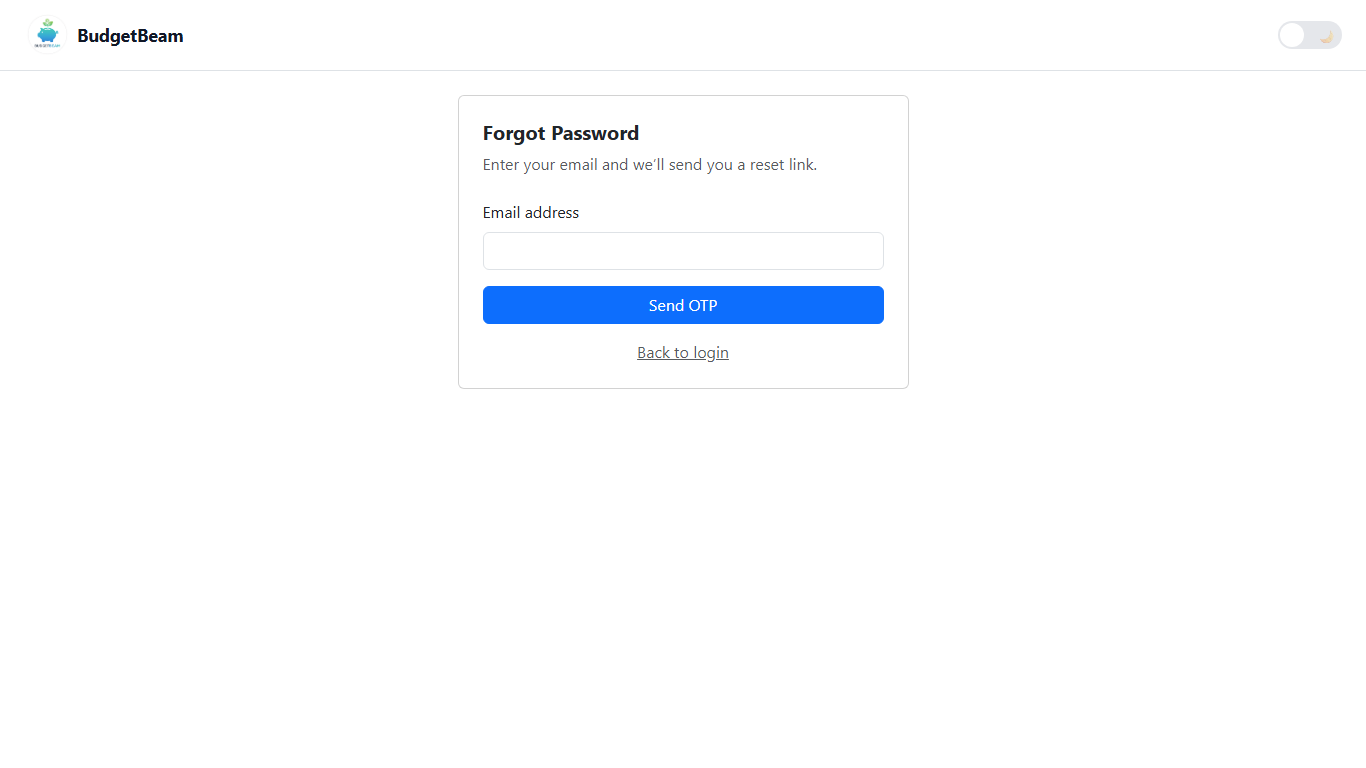
\includegraphics[width=0.85\textwidth]{forgot_password_ui.png}
    \caption{Budgetbeam Password Recovery}
\end{figure}

\textbf{Core Application Interfaces:}
\begin{itemize}
    \item \textbf{Dashboard UI:} A centralized view presenting the current month's total budget, actual spending, and most active categories.
    \item \textbf{Budget Entry UI:} A modal-driven interface for defining category allocations with real-time validation.
    \item \textbf{Expense Log UI:} A searchable, paginated table of all historical expenditures.
\end{itemize}

\begin{figure}[h!]
    \centering
    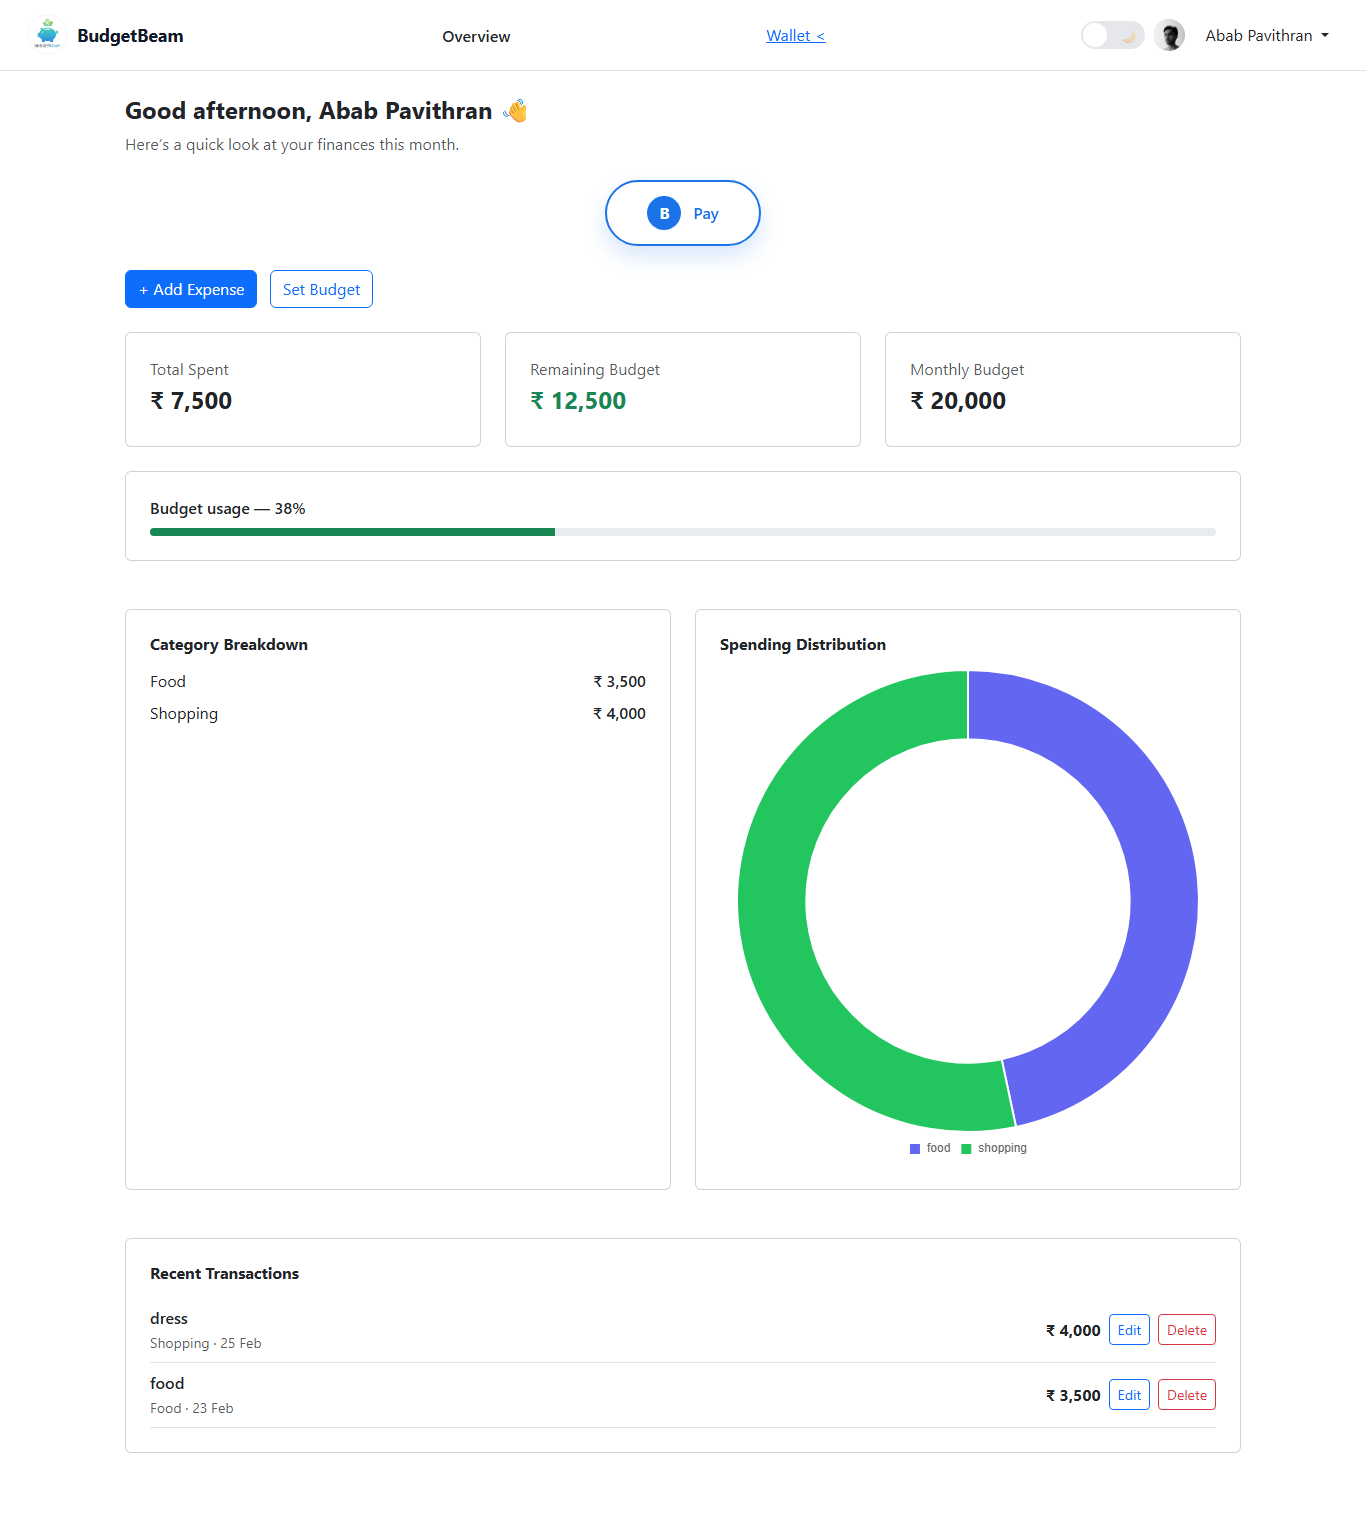
\includegraphics[width=0.85\textwidth]{dashboard_ui.png}
    \caption{Budgetbeam Live Dashboard Interface}
\end{figure}

\begin{figure}[h!]
    \centering
    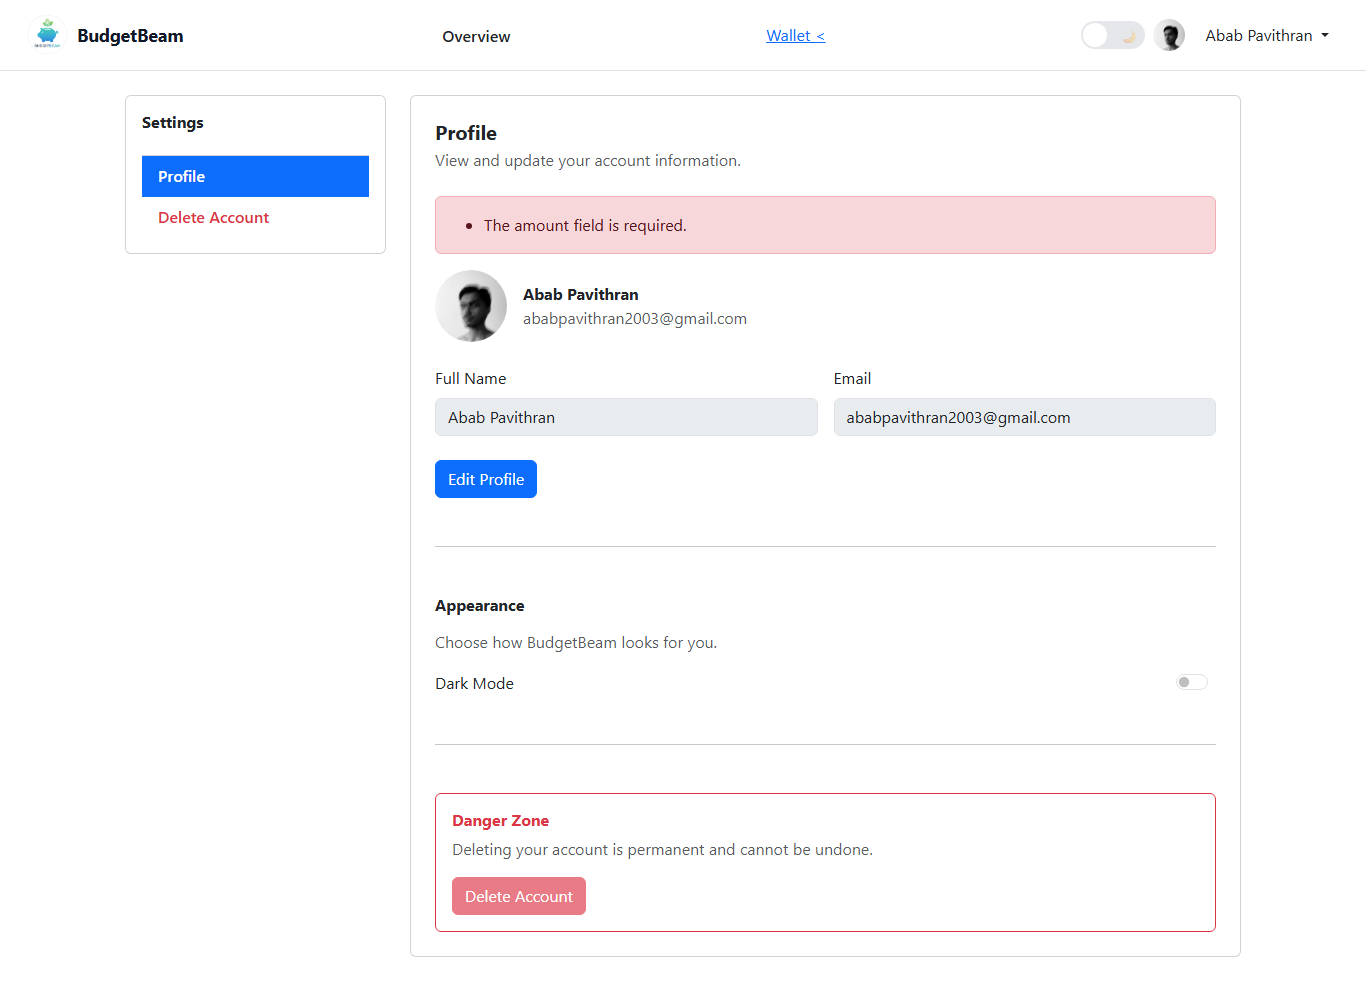
\includegraphics[width=0.85\textwidth]{wallet_ui.png}
    \caption{Secure Wallet Payment Interface}
\end{figure}

\begin{figure}[h!]
    \centering
    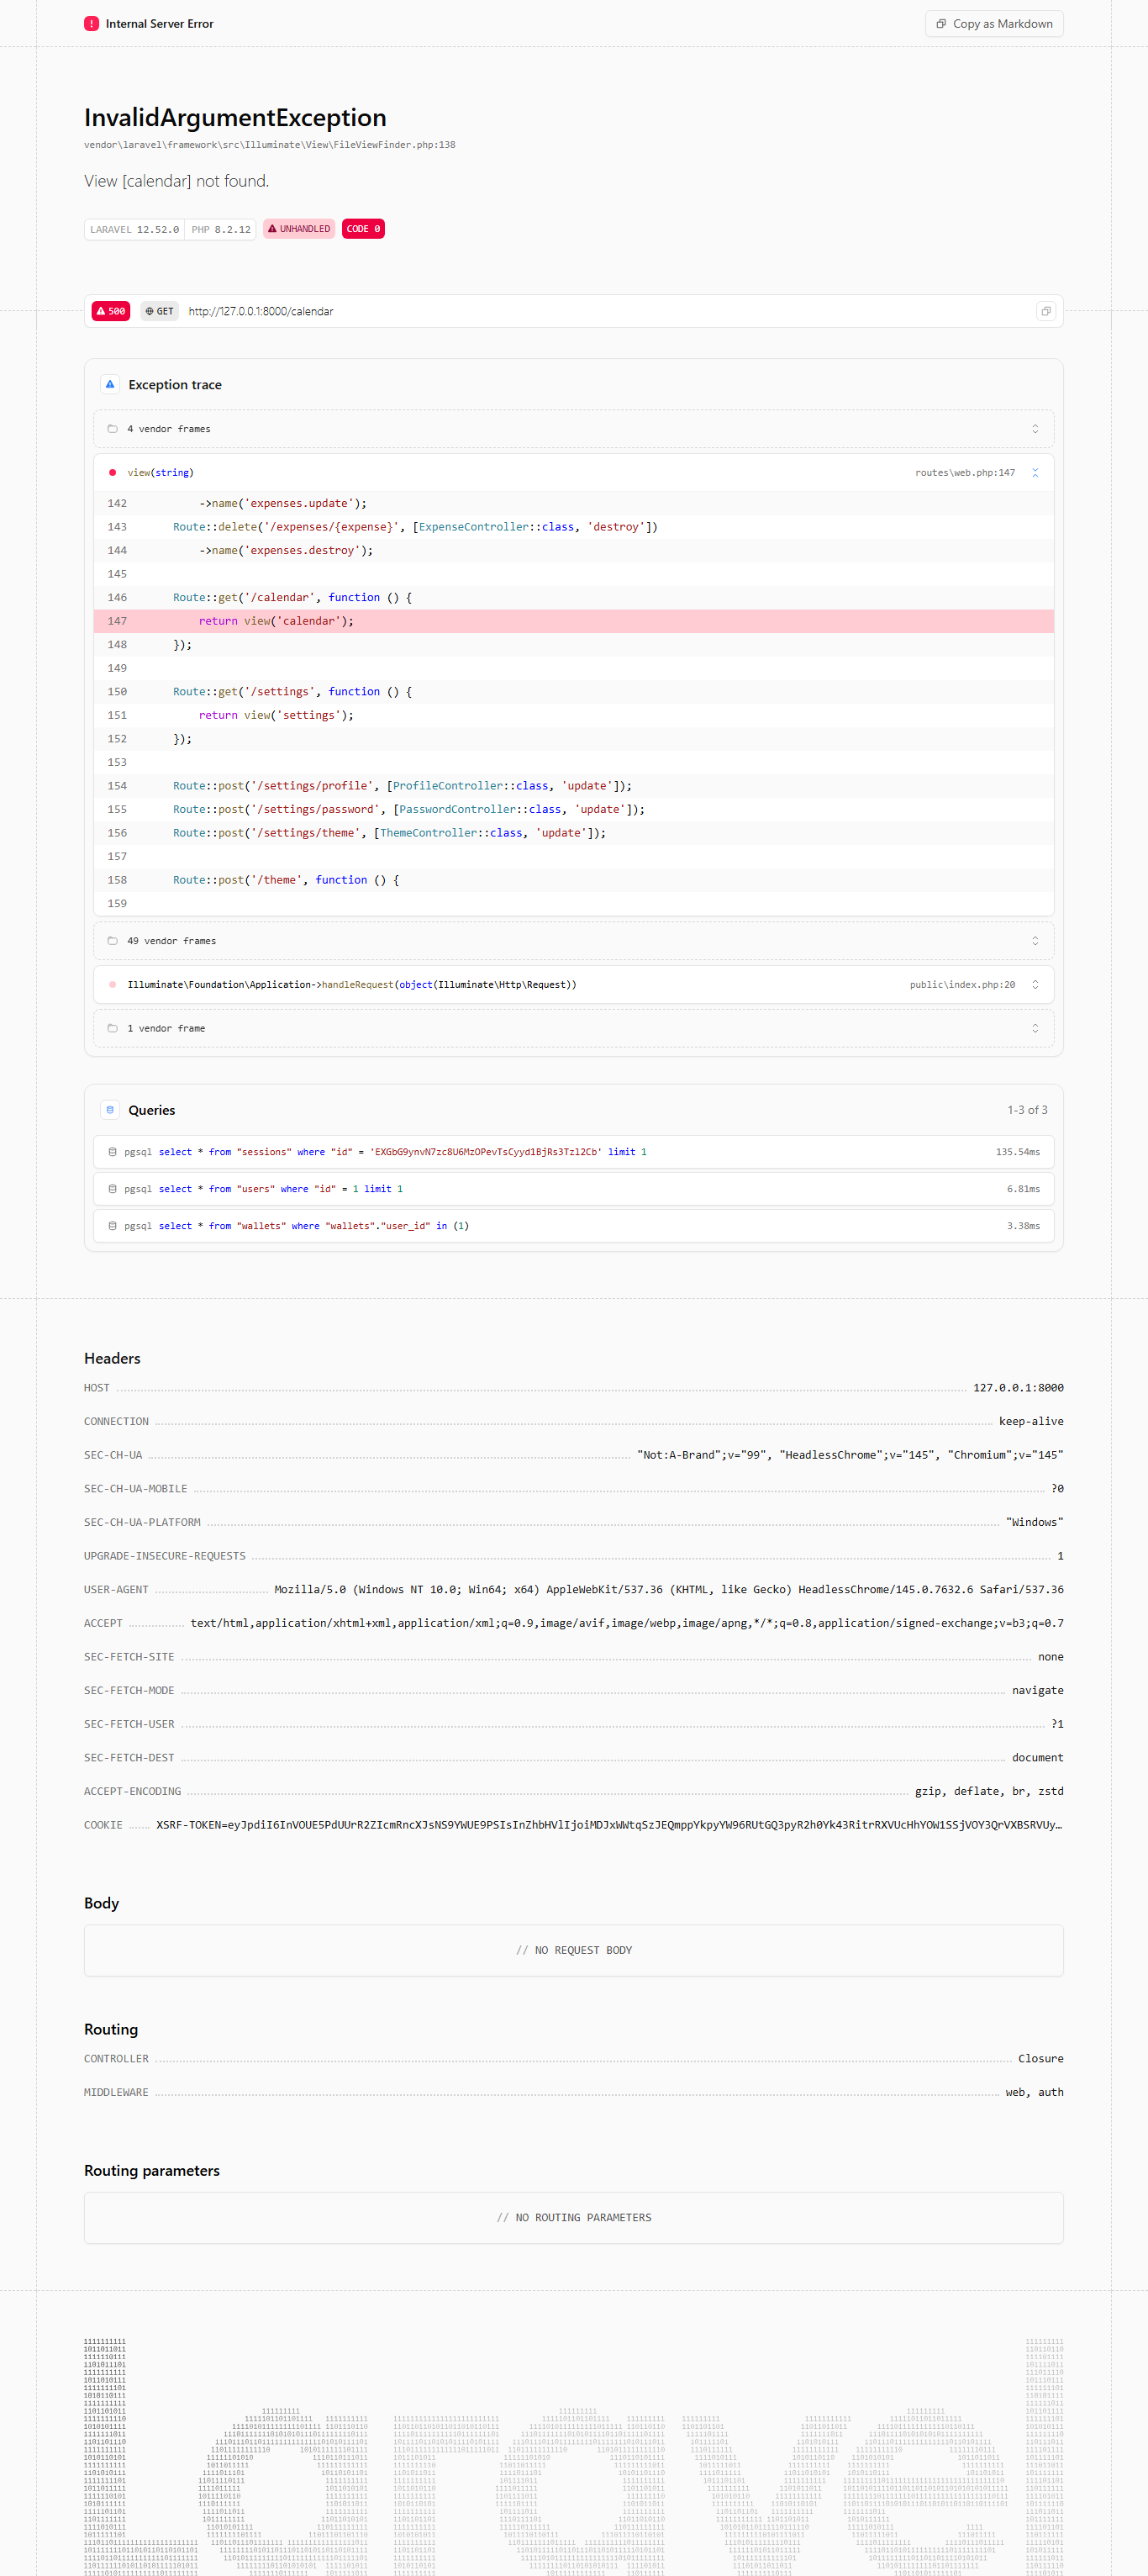
\includegraphics[width=0.85\textwidth]{calendar_ui.png}
    \caption{Interactive Expense Calendar Interface}
\end{figure}

\begin{figure}[h!]
    \centering
    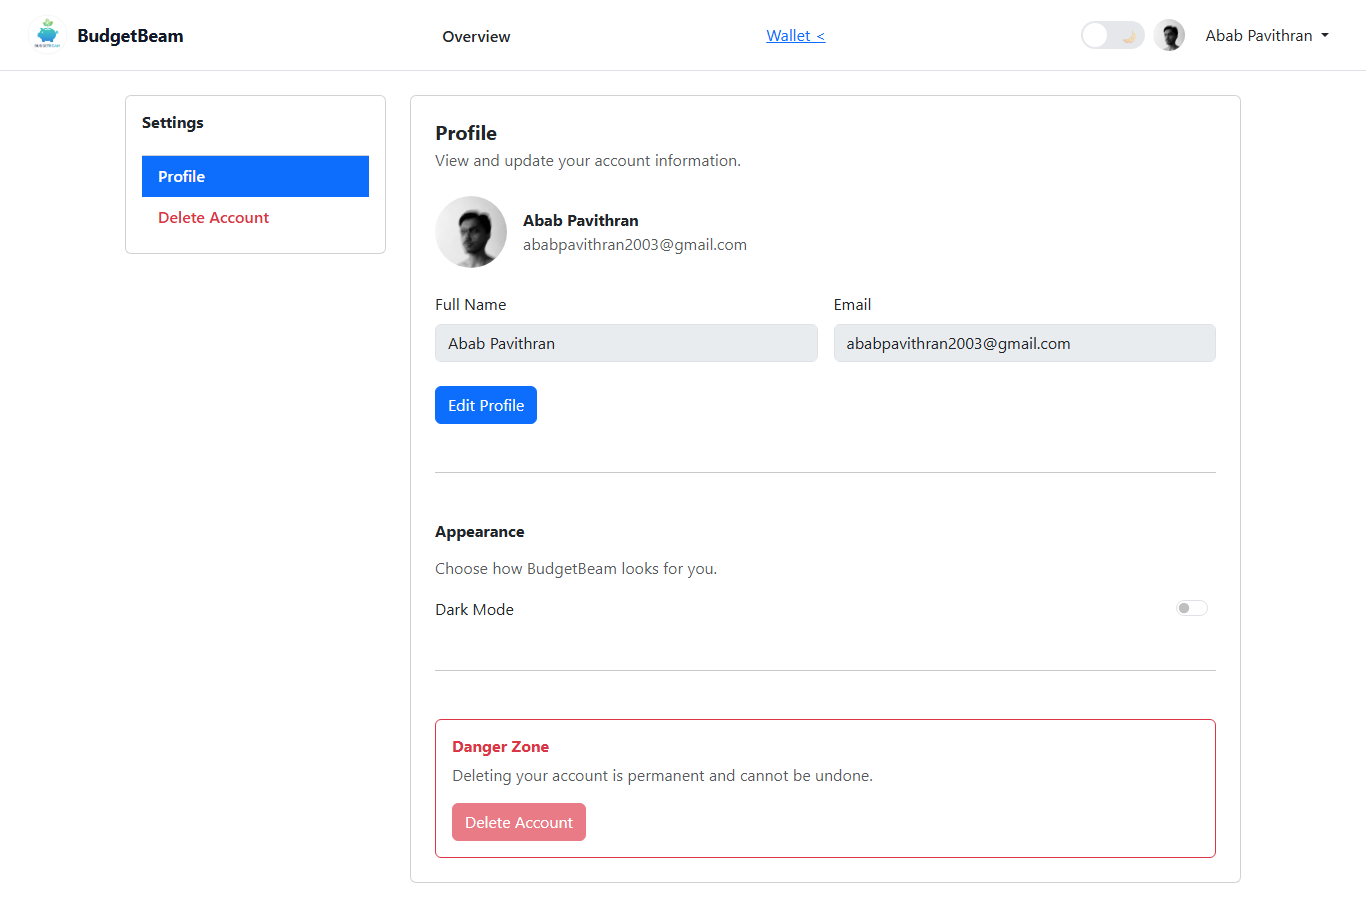
\includegraphics[width=0.85\textwidth]{settings_ui.png}
    \caption{User Profile Settings Interface}
\end{figure}

\clearpage
\section{System Architecture Diagram}
\begin{figure}[h!]
    \centering
    \caption{Budgetbeam System Architecture}
    
\includegraphics[width=\textwidth]{architecture.png}
\end{figure}

\section{Database Design}
The relational schema consists of 13 tables precisely mirroring the actual Budgetbeam database architecture.

\subsection{Core Application Tables}
\begin{longtable}{|l|l|p{7.5cm}|}
\caption{users Table Schema} \\
\hline
\textbf{Field Name} & \textbf{Data Type} & \textbf{Description} \\ \hline
id & BigInt & Primary Key, Auto-increment \\ \hline
name & String & The user's full name \\ \hline
email & String & Unique email address \\ \hline
email\_verified\_at & Timestamp & Nullable \\ \hline
password & String & Hashed password \\ \hline
remember\_token & String & Nullable \\ \hline
role & String & User permission level \\ \hline
theme & String & UI preference \\ \hline
avatar & String & Nullable avatar path \\ \hline
profile\_photo\_path & String & Nullable \\ \hline
monthly\_budget & Decimal(10,2) & Nullable limit \\ \hline
alert\_50\_sent & Boolean & Nullable flag \\ \hline
alert\_90\_sent & Boolean & Nullable flag \\ \hline
alert\_100\_sent & Boolean & Nullable flag \\ \hline
created\_at, updated\_at & Timestamp & Record timestamps \\ \hline
\end{longtable}

\begin{longtable}{|l|l|p{7.5cm}|}
\caption{expenses Table Schema} \\
\hline
\textbf{Field Name} & \textbf{Data Type} & \textbf{Description} \\ \hline
id & BigInt & Primary Key \\ \hline
user\_id & BigInt & FK referencing users \\ \hline
title & String & Expense title \\ \hline
amount & Decimal(10,2) & Expenditure amount \\ \hline
category & String & Category name \\ \hline
expense\_date & Date & Date of transaction \\ \hline
note & String & Nullable details \\ \hline
created\_at, updated\_at & Timestamp & Record timestamps \\ \hline
\end{longtable}

\begin{longtable}{|l|l|p{7.5cm}|}
\caption{wallets Table Schema} \\
\hline
\textbf{Field Name} & \textbf{Data Type} & \textbf{Description} \\ \hline
id & BigInt & Primary Key \\ \hline
user\_id & BigInt & FK referencing users \\ \hline
balance & Decimal(10,2) & Default 0 \\ \hline
created\_at, updated\_at & Timestamp & Record timestamps \\ \hline
\end{longtable}

\begin{longtable}{|l|l|p{7.5cm}|}
\caption{wallet\_transactions Table Schema} \\
\hline
\textbf{Field Name} & \textbf{Data Type} & \textbf{Description} \\ \hline
id & BigInt & Primary Key \\ \hline
wallet\_id & BigInt & FK referencing wallets \\ \hline
type & Enum & 'credit' or 'debit' \\ \hline
amount & Decimal(10,2) & Transaction value \\ \hline
description & String & Nullable details \\ \hline
created\_at, updated\_at & Timestamp & Record timestamps \\ \hline
\end{longtable}

\subsection{Authentication \& Security Tables}
\begin{longtable}{|l|l|p{7.5cm}|}
\caption{password\_otps Table Schema} \\
\hline
\textbf{Field Name} & \textbf{Data Type} & \textbf{Description} \\ \hline
id & BigInt & Primary Key \\ \hline
email & String & User email address \\ \hline
otp & String & One-Time Password \\ \hline
expires\_at & Timestamp & Expiry date/time \\ \hline
created\_at, updated\_at & Timestamp & Record timestamps \\ \hline
\end{longtable}

\begin{longtable}{|l|l|p{7.5cm}|}
\caption{password\_reset\_tokens Table Schema} \\
\hline
\textbf{Field Name} & \textbf{Data Type} & \textbf{Description} \\ \hline
email & String & Primary Key \\ \hline
token & String & Verification token \\ \hline
created\_at & Timestamp & Nullable \\ \hline
\end{longtable}

\begin{longtable}{|l|l|p{7.5cm}|}
\caption{sessions Table Schema} \\
\hline
\textbf{Field Name} & \textbf{Data Type} & \textbf{Description} \\ \hline
id & String & Primary Key \\ \hline
user\_id & BigInt & FK referencing users (nullable) \\ \hline
ip\_address & String(45) & Nullable IP \\ \hline
user\_agent & Text & Nullable \\ \hline
payload & LongText & Serialized session \\ \hline
last\_activity & Integer & Unix timestamp \\ \hline
\end{longtable}

\subsection{Framework \& Infrastructure Tables}
\begin{longtable}{|l|l|p{7.5cm}|}
\caption{migrations Table Schema} \\
\hline
\textbf{Field Name} & \textbf{Data Type} & \textbf{Description} \\ \hline
id & Integer & Primary Key \\ \hline
migration & String & Migration filename \\ \hline
batch & Integer & Batch run number \\ \hline
\end{longtable}

\begin{longtable}{|l|l|p{7.5cm}|}
\caption{jobs Table Schema} \\
\hline
\textbf{Field Name} & \textbf{Data Type} & \textbf{Description} \\ \hline
id & BigInt & Primary Key \\ \hline
queue & String & Queue name \\ \hline
payload & LongText & Job payload \\ \hline
attempts & TinyInt & Count \\ \hline
reserved\_at & Integer & Nullable timestamp \\ \hline
available\_at & Integer & Timestamp \\ \hline
created\_at & Integer & Timestamp \\ \hline
\end{longtable}

\begin{longtable}{|l|l|p{7.5cm}|}
\caption{job\_batches Table Schema} \\
\hline
\textbf{Field Name} & \textbf{Data Type} & \textbf{Description} \\ \hline
id & String & Primary Key \\ \hline
name & String & Batch name \\ \hline
total\_jobs & Integer & Count \\ \hline
pending\_jobs & Integer & Count \\ \hline
failed\_jobs & Integer & Count \\ \hline
failed\_job\_ids & LongText & Serialized IDs \\ \hline
options & MediumText & Nullable \\ \hline
cancelled\_at, created\_at, finished\_at & Integer & Timestamps \\ \hline
\end{longtable}

\begin{longtable}{|l|l|p{7.5cm}|}
\caption{failed\_jobs Table Schema} \\
\hline
\textbf{Field Name} & \textbf{Data Type} & \textbf{Description} \\ \hline
id & BigInt & Primary Key \\ \hline
uuid & String & Unique Identifier \\ \hline
connection & Text & Connection name \\ \hline
queue & Text & Queue name \\ \hline
payload & LongText & Job payload \\ \hline
exception & LongText & Error trace \\ \hline
failed\_at & Timestamp & Default Current Timestamp \\ \hline
\end{longtable}

\begin{longtable}{|l|l|p{7.5cm}|}
\caption{cache Table Schema} \\
\hline
\textbf{Field Name} & \textbf{Data Type} & \textbf{Description} \\ \hline
key & String & Primary Key \\ \hline
value & MediumText & Cached data \\ \hline
expiration & Integer & Expiry Unix Timestamp \\ \hline
\end{longtable}

\begin{longtable}{|l|l|p{7.5cm}|}
\caption{cache\_locks Table Schema} \\
\hline
\textbf{Field Name} & \textbf{Data Type} & \textbf{Description} \\ \hline
key & String & Primary Key \\ \hline
owner & String & Lock owner \\ \hline
expiration & Integer & Expiry Unix timestamp \\ \hline
\end{longtable}

\section{UML Documentation}
\subsection{Class Diagram}

\includegraphics[width=\textwidth]{class.png}
\subsection{Entity-Relationship (ER) Diagram}
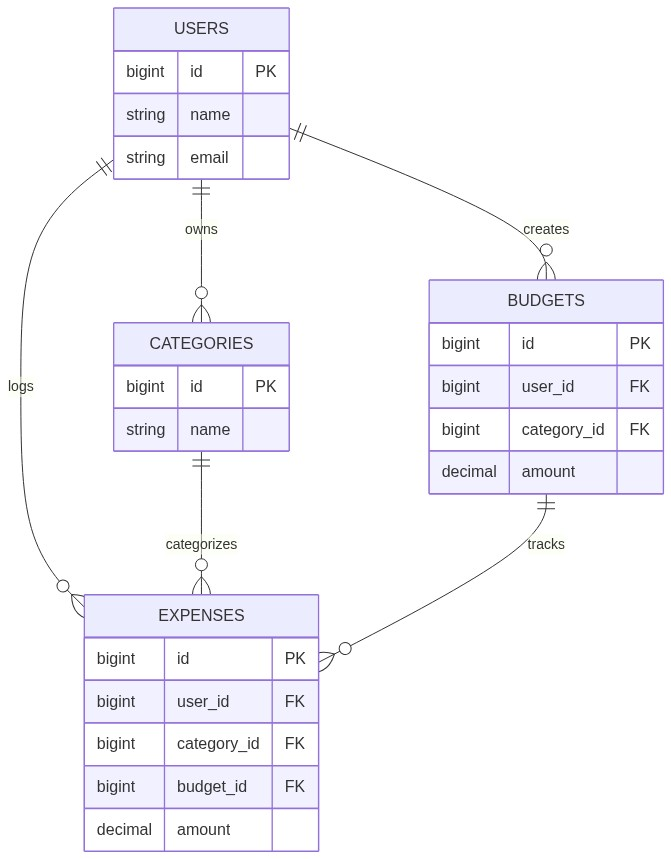
\includegraphics[width=\textwidth]{er.png}
\subsection{Sequence Diagram (Expense Logging)}

\includegraphics[width=\textwidth]{sequence.png}

\section{Project Development Pipeline}
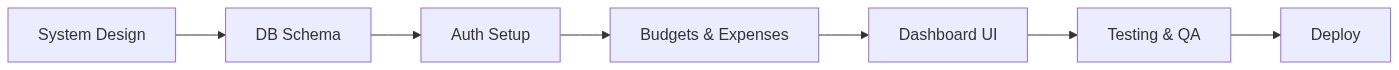
\includegraphics[width=\textwidth]{pipeline.png}
